\documentclass{llncs}

\usepackage{makeidx}  % allows for indexgeneration

\usepackage{graphics, graphicx, xcolor}
\usepackage{amsmath}
%\usepackage[square]{natbib}
\usepackage{cite}
\usepackage[hidelinks, colorlinks, linkcolor={red},citecolor={blue}, urlcolor={blue}, backref=section]{hyperref}

\usepackage{times}

\newcommand{\authcmt}[2]{\textcolor{#1}{#2}}
\newcommand{\yuncong}[1]{\authcmt{red}{[YC: #1]}}
\newcommand{\yoav}[1]{\authcmt{blue}{[YF: #1]}}

\begin{document}

%\abovedisplayskip=2pt 
%\abovedisplayshortskip=1pt
%\belowdisplayskip=2pt 
%\belowdisplayshortskip=1pt
%\textfloatsep=5pt
%\intextsep=3pt

%
%\mainmatter              % start of the contributions
%
\title{Robust Landmark Detection for Alignment of Mouse Brain Section Images}
%
\titlerunning{Robust Landmark Detection for Mouse Brain Images}  % abbreviated title (for running head)
%                                     also used for the TOC unless
%                                     \toctitle is used
%
\author{Yuncong Chen, David Kleinfeld, Martyn Goulding \and Yoav Freund}
%
\authorrunning{Yuncong Chen et al.} % abbreviated author list (for running head)
%
%%%% list of authors for the TOC (use if author list has to be modified)
% \tocauthor{Yuncong Chen, Yoav Freund}
%
\institute{Department of Computer Science and Engineering, \\University of California, San Diego, La Jolla, CA 92122, USA}

\maketitle              % typeset the title of the contribution
\begin{abstract}

Brightfield and fluorescent imaging of whole brain sections is a fundamental tool in anatomical studies on brain functions. As sectioning and imaging become more efficient, there is an increasing need to automate the post-processing of sections for alignment and three dimensional visualization. There is a further need to facilitate the development of a digital atlas, i.e. a brain-wide map annotated with cell type and tract tracing data, which serves as the underpinning for circuits analysis as well as for quantitative analysis of phenotypical variation. Currently, construction of such maps requires tedious human labelling. In this work we describe the first steps in developing a semi-automated system to construct a histology atlas of mouse brainstem that combines atlas-guided annotation, landmark-based registration and atlas generation in an iterative framework. 
%This atlas stores landmark models, uses them to detect landmarks from new images and maps the images onto the atlas's standardized coordinate system; meanwhile, the models in the atlas are updated based on newly registered images.
In particulcar, we describe an unsupervised approach for identifying and matching region and boundary landmarks, based on modelling texture. Experiments show that the detected landmarks correspond well with brain structures, and matching is robust under distortion. The results serve as a promising basis for the next stage of registration and atlas building.

\keywords{landmark detection, atlas building, mouse brain, registration, automated annotation}

\end{abstract}
%

\section{Introduction}

In this paper we describe a method for the automatic detection of landmarks in histology images of mouse brain sections. The purpose is to facilitate image registration and atlas generation. By aligning images of nissl and fluorescent-stained brain sections, we aim to create a 3D digital atlas for the mouse brainstem, which incorporates cell type, tract tracing and other physiological data. The novelty of our method is in the use of unsupervised learning to find regions with distinct texture and clear boundaries, which reduces time-consuming human labelling.

Figure x shows a typical image of nissl-stained mouse brainstem section. Although the brainstem does not have salient edges like the cortex, it contains many compact neuron clusters (nuclei) and striated regions (fiber tracts). Both types of structure have distinct texture that can be detected and modelled.

In this work, We use semi-supervised learning to create a library of texture and shape detectors. They can be applied to identify landmarks from new images and also be updated by incorporating new data. This is at the center of our vision of integrating atlas-guided annotation, landmark-based registration and atlas generation into an iterative framework.

% represent appearance landmark using binarized gradient orientation histograms and boundary landmark using curvature, and use MRF for registration.

% \cite{song20133d} proposing an unsupervised content classification method, which automatically identifies common content classes from differently stained histology image pair

%Maximizing mutual information 

%Brightfield and fluorescent imaging is a fundamental tool in mouse brain studies. As sectioning and image acquisition become more efficient, there is a need to facilitate the development of a digital atlas, i.e. a brain-wide map annotated with anatomical structures as well as cell type, tract tracing and physiological data. Such map serves as the underpinning of brain circuit analysis and quantitative analysis of phenotypical variation.

%It is interesting to note that, on the one hand, if the specimen is labelled, annotated atlas facilitates landmark-based registration. On the other hand, atlas-guided annotation requires the specimen be brought into registration with the atlas first, which is often done by manually picking landmarks. In either case, time-consuming human labelling is needed. To alleviate this bottleneck, we propose to use machine learning to model the landmarks with appearance features. By training landmark detectors and storing them in the atlas, landmarks can be automatically identified in new images. These landmarks guide both intra-specimen and specimen-atlas registration. Landmark models are then updated based on registered new images.

%This paper describes a first step towards building a three-dimensional histology atlas for mouse brainstem. The system will integrate atlas-guided annotation, landmark-based registration and atlas generation into an iterative framework, allowing the atlas to continue improving itself using new data. The particular aspect described in this paper is the automatic detection and modelling of brainstem landmarks.

%making it particularly suitable for processing a large number of specimens in an incremental fashion. 
%Most existing histology atlases generation approaches align the histology series to an MRI template volume, often based on manually picked landmarks. In comparison, we aim to construct the atlas using only histology images. We also aim to minimize human labelling by using unsupervised algorithms to detect and model salient brain regions.

%The atlas incorporates registered specimens, leading to better landmark models, which in turn leads to more accurate annotation of new specimens, and thus more accurate registration.

%The cyclic dependence now enables a self-improving system.

%By automatically detecting landmarks, we not only reduce human labelling effort by providing suggestions 

%One crucial component in our system is identifying the landmarks. Until the region models are trained with sufficiently many examples, the system must obtain the annotation in other ways. Having human labellers do the annotation is time-consuming. In this paper, we propose an automatic approach for identifying potential landmarks including significant regions and boundaries.

%Unlike the cerebrum and the cerebellum, where high-contrast cortex presents clear edges, the brainstem mostly contains nuclei, which are compact neuron clusters with homogeneous and distinct texture, and
%%For example, Figure 1 shows the facial motor nucleus. 
%%Neurons in each nucleus have similar size, shape and stain sensitivity, often also demonstrating uniform density and particular directionality. This gives each nuclei a distinctive texture, allowing them to be robustly identified from the image. The fact that they are well localized also makes them perfect landmarks for registration. 
%fiber tracts, which are recognizable for their striated texture. 
%%In particular, the directionality of a tract serves as an important feature of the landmark.
%This motivates our algorithm to model texture, and detect landmarks including both compact regions and boundaries.

The remaining of this paper is organized as the follows. Section 2 describes how we represent textures using Gabor filters and superpixels. Section 3 and 4 explains how we identify potential landmark regions based on texture distinctiveness. Section 5 describes how we detect stable boundary segments to complement region landmarks. Section 6 describes how landmarks are matched between sections.

%Our method is not a segmentation algorithm. As we are only interested in identifying and modelling a small proportion of the image that are of interest to the researcher.

%We only apply our method to nissl-stained brain sections. For building the atlas, we need to make sure it is applicable to fluorescent images.

\section{Related Work}


Currently, histology atlas is most often constructed by aligning the histology series to an MRI template volume. This often require experimentalist to manually identify landmarks.

The Allen Brain Atlas\cite{lein2007genome} and Waxholm Space \cite{lee2005standard} construct the histology atlas by aligning histology series to an MRI template volume \cite{yushkevich20063d}.


based on a combination of high-frequency sectionto-section
histology registration with low-frequency histology to (ex-cranio) MRI registration (Yushkevich, 


An atlas is typically constructed by mapping image series of different studies to a common coordinate system, and aggregating the information. 
Images of different modalities or specimens stained for different targets can be superimposed. For example, the Allen Mouse Brain Atlas\cite{lein2007genome} computes the expression energy of different genes by collecting statistics from in-situ hybridization images of all the studies. 
In other cases, inter-specimen variation is interested. For example, the Waxholm Space atlas\cite{lee2005standard} provides an anatomical probability map that gives the probability of each voxel belonging to a particular anatomical structure. The probabilities are computed from a large number of co-registered specimens.


Currently most histology atlases are constructed by registering histology series to an MRI template volume. This often requires experimentalist to manually identify landmarks in each section, which is labor intensive. 
In contrast, our method would require the experimentalist to validate our library of texture and shape detectors. Once those have been validated, the process is completely automatic.


There has been much work on reconstructing 3D volume from histology sections. Intensity-based methods \cite{ourselin2001reconstructing, roberts2012toward} uses block-matching to compute a regularized displacement field. Other methods rely on detecting gradients in the image, and compute alignment by smoothing high-gradient edges \cite{cifor2011smoothness, bagci2010automatic, haber2006intensity}. The level of details in histology images also motivates the use of more elaborate descriptors, including SIFT \cite{sun2012nearly}, binarized gradient orientation histogram \cite{kurkure2011landmark} and bag of multiple types of features \cite{cruz2011visual}. 


\section{Representing Texture using Histograms of Gabor Textons} 

%It captures responses on different orientations and scales.
%
%Local Spectral histograms
%
%Other descriptors that have been applied to histology images include local binary patterns, grey-level co-occurrence matrix, intensity histogram and SIFT. [Tu]
%
%Textons are proposed in \cite{leung2001representing}

Images are first filtered using Gabor filters\cite{jain1990unsupervised, clausi2000designing} with 9 orientations and 11 scales, resulting in 99 dimensional feature vectors. We reduce the data by quantizing these feature vectors into 100 clusters using K-Means. Clusters with close centroids are then merged, and the final cluster centroids are the textons. In our experiment, we have 14 textons.

%\begin{figure}
%\caption{Gabor Filters}
%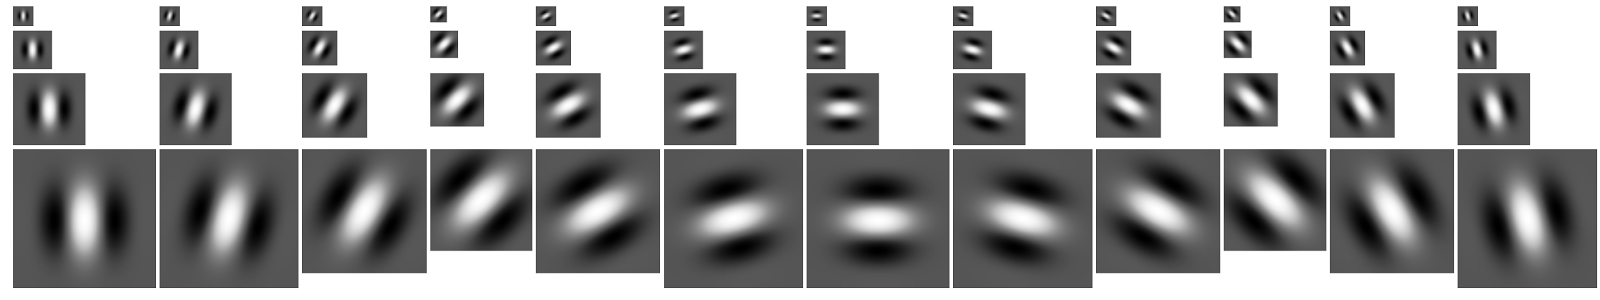
\includegraphics[width=0.5\textwidth]{../figures/gabor}
%\end{figure}

We further reduce the data by describing texture at the level of superpixels. For each superpixel, texture is represented by the histogram of the textons it contains (Figure \ref{fig:TextonHistComparison}). We denote the texton histogram of the $i$'th superpixel by $h_i$. Superpixels are obtained using the SLIC algorithm \cite{achanta2012slic}.

Since different sections may be oriented at different angles, 
%and in order for two identical but slightly rotated textures to match, 
we need the features to be rotation-invariant. For this purpose, before doing K-Means, we compute the energy distribution over orientations for each Gabor feature vector, and shift all feature vectors such that the modes of the directional energy distributions are aligned. In this way, the texture is decoupled from directionality.

\begin{figure}
	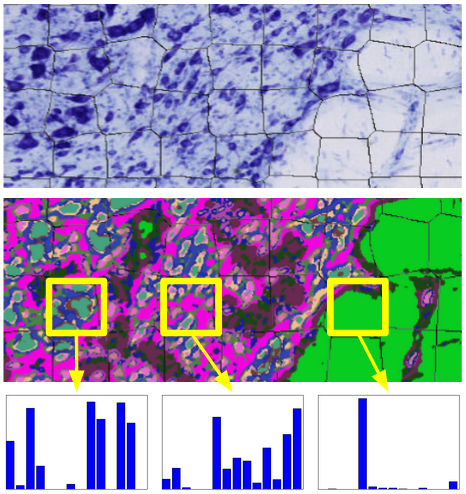
\includegraphics[width=.5\textwidth]{../figures/TextonHistComparisonWithArrows.png}
	\caption{Top: part of the original image with superpixels overlaid. Middle: texton map of the same area. Bottom: texton histograms of three superpixels with different textures.}
	\label{fig:TextonHistComparison}
\end{figure}

%Note that the directionality is still useful, particularly for describing fiber tracts.

\section{Evaluating Region Significance using Statistical Test}

We define a region landmark as a connected set of superpixels. Before describing how to find significant regions, we need a scoring function that evaluates the significance of a region. We propose the significance score, $F(S)$, of a region $S$, to be a linear combination of three terms. 

The first term is the distinctiveness of this region's texture, or in other words, how different its texture is from the surrounds. Since textures are represented as histograms, we formulate this problem as a statistical test on whether the region's average texton histogram and the texton histograms of the surrounding superpixels are sampled from the same distribution. We employ the chi-squared test for independence and the resulting p-value serves as a quantitative measure of the distinctiveness. The smaller the p-value, the more significant the region is. Since a region often has neighbours with different textures, the test is made between the region's histogram and that of every surrounding superpixel. To be conservative, the largest p-value among all tests is used. Denote the set of surrounding superpixels by $T(S)$, the first term is,
$$F^{cont}(S) = - \max_{j\in T(S)} pval(h_S, h_j)$$
where $pval(\cdot,\cdot)$ is the p-value of applying the chi-square test for independence to two histograms.

The second term is the texture homogeneity within the region, defined as the mean p-value of chi-square tests between all superpixels in the region and the region's average:
$$F^{coh}(S) = \frac{1}{|S|} \sum_{i\in S} pval(h_S, h_i)$$

The third term stems from the fact that most region landmarks have compact shapes. A common measure for the compactness of a closed curve is the isoperimetric quotient, defined as the enclosing area divided by the square of the circumference. We use the number of surrounding superpixels as a proxy for the circumference, and the number of superpixels in the region as that for the area. Small 
$$F^{comp}(S) = \frac{|T(S)|}{|S|^2}$$

The overall significance score $F(S) = F^{cont}(S) + F^{coh}(S) + F^{comp}(S)$.


\section{Finding Significant Regions with Region Growing and Clustering}

To find potential regions, we perform region growing for every superpixel. Starting with a singleton containing the seed superpixel, this greedy procedure considers all neighbours of the current set, and iteratively adds the one whose texture is closest to the current region's texture, measured by the $\chi^2$ distance between texton histograms. The growing stops when the region reaches 10\% of the total area. Eventually, the region at the point when the significance score is the largest is returned. Figure \ref{fig:RegionGrowing} shows examples of this procedure.
\begin{figure}
	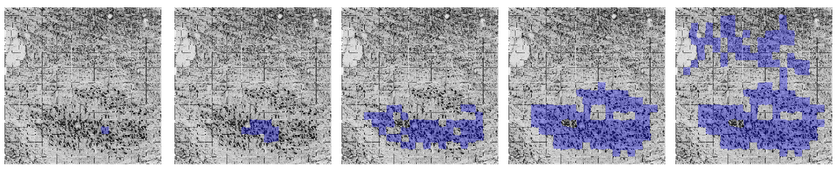
\includegraphics[width=\textwidth]{../figures/RegionGrowingPicsOnly.png}
	\caption{Regions during growing, from left to right, at iteration 1, 10, 50, 96 (most significant), 150 (last iteration).} %Below it are plots of the significance score and the three terms.}
	\label{fig:RegionGrowing}
\end{figure}

%The termination criteria is a threshold on the histogram dissimilarity between the newly added superpixel and the set average. Instead of using a pre-determined threshold, we over-grow the region until its size reaches 10\% of the total area, and record this dissimilarity at every iteration. The dissimilarity would be the largest when the growing incorporates a superpixel that is the most different in hindsight, and thus the region just before this point is returned as the result of growing. This maximum dissimilarity can be used as a measure for the contrast, since every added superpixel is lower than this value.

We call the set of superpixels that grows from a seed superpixel $k$ the \textit{region proposal} of the seed, denoted by $S_k$. If a region has distinct texture, the proposals of superpixels inside this region should be very similar, while proposals from within an inhomogeneous region are random (see Figure \ref{fig:ConsistentProposals}). In other words, the region proposals form clusters. The denser a cluster is, the more distinctive the region it represents. Using Jaccard index as pairwise distance, we group the region proposals using hierarchical clustering. Then within each group whose size is large enough, we select the proposal with the highest significance score to be the representative of that group. All representative proposals are ranked according to their significance scores. 

%Figure \ref{fig:TopRegions} shows the top 20 region proposals detected in two consecutive sections. Many nuclei are detected.

\begin{figure}
	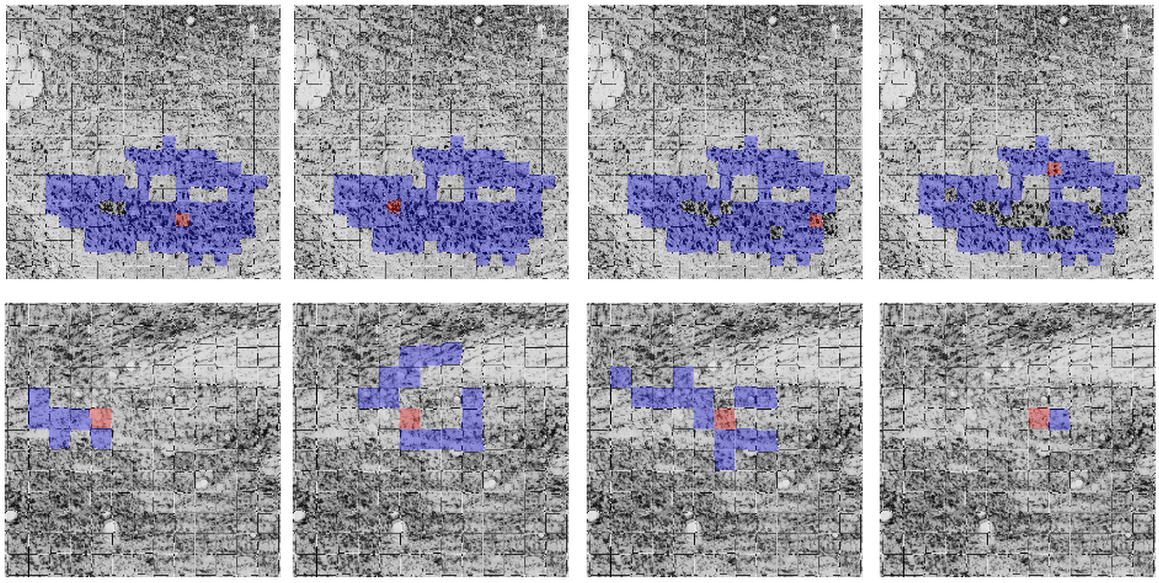
\includegraphics[width=\textwidth]{../figures/ProposalsGoodAndBad.png}
	\caption{The first row shows the region proposals of four different seeds (in red) in the facial motor nucleus. They are very similar. The second row shows the proposals of four neighboring seeds in an inhomogeneous region. They are very different.} %Below it are plots of the significance score and the three terms.}
	\label{fig:ConsistentProposals}
\end{figure}

%\begin{figure}[h]
%	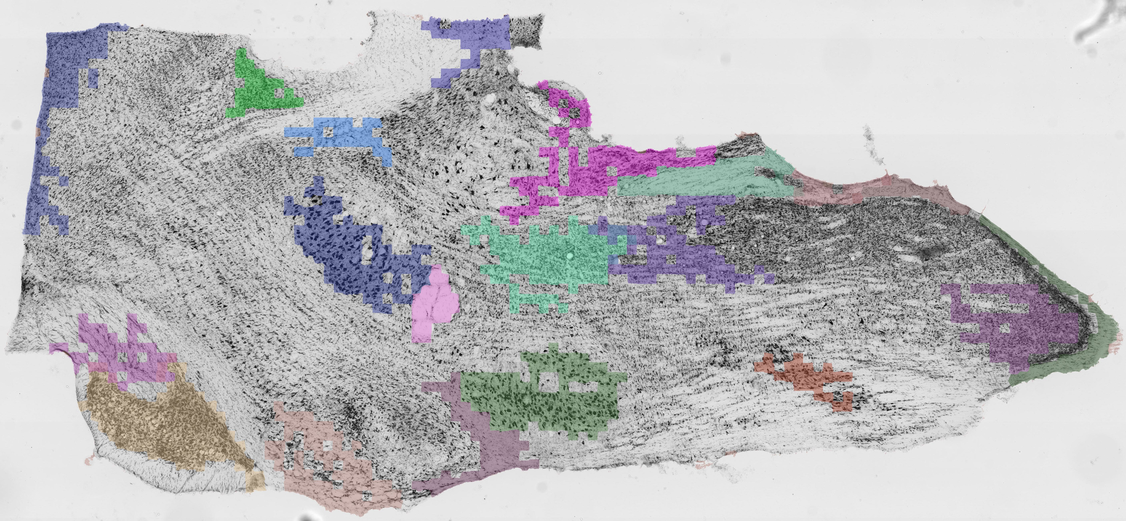
\includegraphics[width=\textwidth]{../figures/RegionsTop20Small.png}
%	\caption{Top 20 significant region proposals.} 
%	\label{fig:TopRegions}
%\end{figure}
 
\section{Identify Robust Boundaries by Region Consensus}

Sometimes a region gradually transitions into neighboring texture on one side, but has a clear boundary on the other side. The method described in the previous section may not capture this inhomogeneous region, but the open boundary is nonetheless a perfect landmark. Figure \ref{fig:RobustBoundaryExample} shows such an example. Notice how much the proposals from seeds in such region vary, but many of them still agree on the clear boundary. This motivates a consensus-based approach for evaluating boundary robustness, in which each region proposal votes for the segments on its boundary.

%Since region growing is sensitive to the seed, 
\begin{figure}
	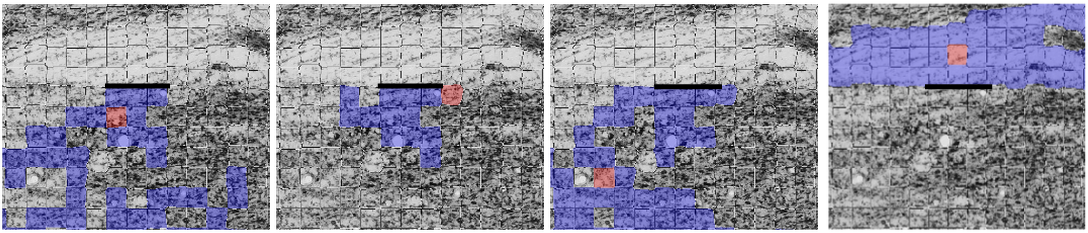
\includegraphics[width=\textwidth]{../figures/RobustBoundaryExampleHighlightLine.png}
	\caption{The three region proposals in an inhomogeneous area are not consistent as a whole, but they all agree on a robust boundary segment (highlighted).}
	\label{fig:RobustBoundaryExample}
\end{figure}

We represent a boundary segment between two superpixels by an ordered tuple $(i,j)$, where $i$ is the interior superpixel and $j$ is the exterior superpixel. We also denote by $\delta S_k$, the set of segments on the boundary of a region proposal $S_k$. 
%We let each region proposal vote for its boundary segments. 
The vote a region proposal casts to a boundary segment depends on how contrasty the segment is, measured by the texture histogram distance between the region's average and the segment's exterior superpixel. We call the set of superpixels that vote for a segment the \textit{supporter set} of the segment, and denote it by $R_{(i,j)} = \{k: (i,j) \in \delta S_k\}$. The total score received by a segment $(i,j)$ is then: 
$$ b_{(i,j)} = \sum_{k \in R(i,j)} \chi^2(h_{S_k}, h_j)$$
%$$ b_{(i,j)} = \sum_{k \in R(i,j)} \frac{\chi^2(h_{S_k}, h_j)}{|S_k|}, $$

We discard segments whose vote is lower than a threshold. Figure \ref{fig:BoundaryMap} shows a vote map. Instead of modelling individual segments, we combine segments with similar supporter sets into groups, again using hierarchical clustering with Jaccard index between supporter sets as pairwise similarity. Each segment group represents a boundary. All boundaries are ranked according to the total vote received by its segments. 

\begin{figure}
	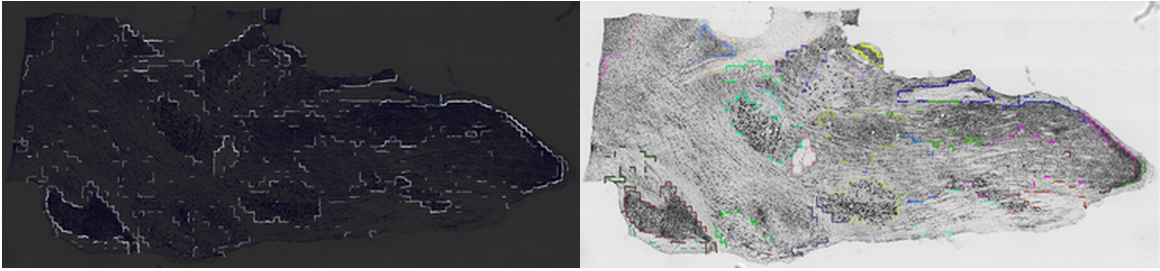
\includegraphics[width=\textwidth]{../figures/BoundariesThreshAndGroupedHorizontal.png}
	\caption{Left: thresholded boundary vote map. Right: grouped boundary segments}
	\label{fig:BoundaryMap}
\end{figure}


\section{Matching Landmarks from Different Sections}

By representing region landmarks using closed boundaries and merging coinciding boundaries, we unify the two types of landmarks into a single set consisting of both open and closed boundaries. In order to use the landmarks for registration, correspondences must be made between them. In this section, we design a distance function for comparing two boundaries. This function is a weighted combination of the differences in four aspects, with weights chosen empirically:
\begin{align*}
D(\mathbf{B}_1, \mathbf{B}_2) = & ~w^{int} D^{int}(\mathbf{B}_1, \mathbf{B}_2) + w^{shape} D^{shape}(\mathbf{B}_1, \mathbf{B}_2)  \\
+ & ~w^{ext} D^{ext}(\mathbf{B}_1, \mathbf{B}_2) 
+ w^{loc} D^{loc}(\mathbf{B}_1, \mathbf{B}_2) 
\end{align*}

The first term is the difference of interior textures. For a region landmark $S$, the interior texture is simply the average texton histogram $h_S$. For a boundary $B$, the interior texture is the average texton histogram of the union of all segments' supporter sets. Denote this union by $Q_B = \cup_{(i,j)\in B} R_{(i,j)}$, then $h^{int}_B = h_{Q_B}$. The difference is computed using the $\chi^2$ distance:
$$D^{int}(\mathbf{B}_1, \mathbf{B}_2) = \chi^2(h^{int}_{B_1}, h^{int}_{B_2})$$

The second term measures the similarity of boundary shapes. We reduce the boundary to a point set consisting of midpoints of the segments. The shape distance between two point sets can be computed using shape context descriptors\cite{belongie2000shape}. The shape context descriptors characterize the organization of other points around each point using a histogram. Two sets of points are matched by finding the minimum bipartite matching, where the edge weights are the chi-square distances between shape context descriptors. The Hungarian algorithm is used to find the minimum matching. The average cost of this matching, is used as the second term:

$$D^{shape}(\mathbf{B}_1, \mathbf{B}_2) = \frac{1}{|M|}\sum_{(i,j), (p,q) \in M(B_1,B_2)} \chi^2(c_{i,j}, c_{p,q})$$ where $M(B_1,B_2)$ is the minimum matching, $c_{i,j}$ and $c_{p,q}$ are the shape context descriptors of segment $(i,j)$ and segment $(p,q)$ respectively.

After the matching is made, we compute the third term, defined as the total distance between exterior textures of all matched segments:
$$D^{ext}(\mathbf{B}_1, \mathbf{B}_2) = \sum_{(i,j), (p,q) \in M(B_1,B_2)} \chi^2(h_j, h_q)$$


The fourth term measures the spatial proximity. This is the thresholded Euclidean distance between the center of mass of the boundaries' midpoint sets:
$$D^{loc}(\mathbf{B}_1, \mathbf{B}_2) = \max(0, \| m_{B_1}, m_{B_2} \|_2 - l)$$
where $m_{B_1}$ and $m_{B_2}$ are the center of mass of boundaries $B_1$ and $B_2$, and $l$ is a tolerance within which the position deviation is not penalized (set to 1 mm in our experiment).

%exterior textures: the symmetric Hausdorff distances between the two sets of exterior distributions. That is, the maximum among the $\chi^2$ distances between each distribution and its closest distribution from the other set.

%shape: the total $\chi^2$ distances of shape context descriptors after the superpixels on two boundaries using dynamic programming. (This is essentially the Shape Distance in Section 5.1 of Belongie's paper)

Using this distance function, we compute the pairwise distances for two sets of landmarks detected from different sections. Two landmarks are matched if they are simultaneously the closest landmark to each another.

\section{Human Supervision}

This system reduces human supervision in annotating brain images. Without any prior annotation, the region landmarks detected by the system can serve as suggestions for significant regions that require annotation. A human labeller then inspects the suggested landmarks. If a landmark is judged to correspond to a real anatomical structure, the human labeller gives it a name and the model of this landmark is stored in the atlas. The human labeler can also manually correct landmarks that are misplaced or create new annotations.
The stored models are compared to the landmarks detected on a new image. If some detected landmarks match the models in the atlas, annotation of these landmarks can be transferred to the new image automatically.

%In addition, both region and boundary landmarks that are matched can be used for correspondence-based registration. This is part of our plan for future work.


\section{Experiments}

\subsection{effectiveness of landmark detection}

We test our algorithm on a series of 30 section images of a nissl-stained mouse brainstem. The images are scanned at 2 microns per pixel, showing individual neuronal cell bodies. Both types of landmarks are detected on all images. For each image we use the top 30 closed boundary and the top 10 open boundary. Figure \ref{fig:TopRegions} shows the landmarks detected from two consecutive sections. Most identifiable nuclei as well as fiber tracts are detected on both sections.

%\begin{figure}
%	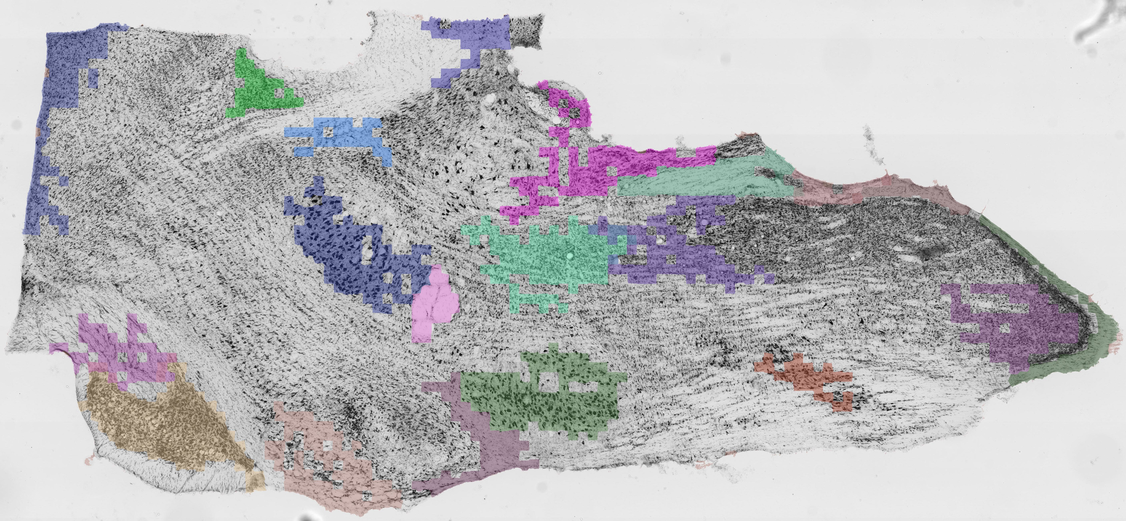
\includegraphics[width=\textwidth]{../figures/Top20Regions_0007.png}
%	\caption{Top 20 boundaries detected in one section}
%	\label{fig:TopRegions}
%\end{figure}

\begin{figure}
	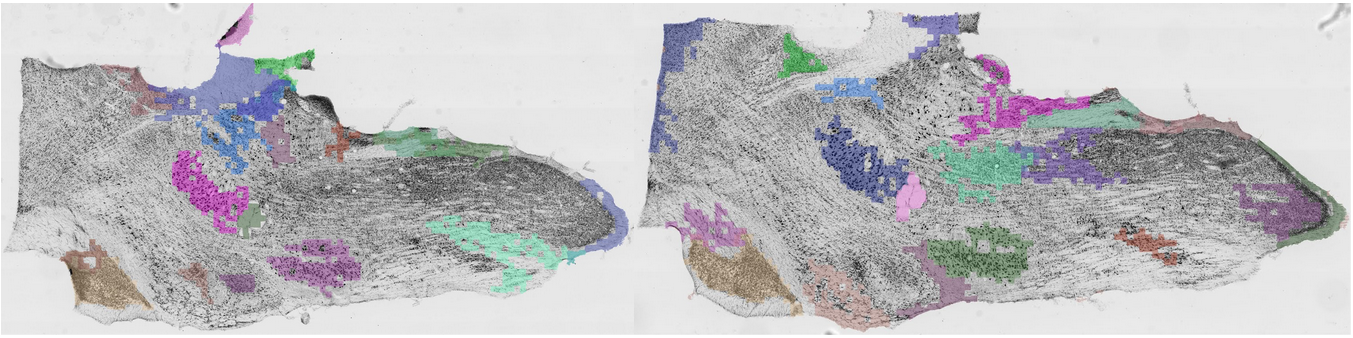
\includegraphics[width=\textwidth]{../figures/TopRegions_0006_0007_Horizontal.png}
	\caption{Top 20 boundaries detected in consecutive sections}
	\label{fig:TopRegions}
\end{figure}

%Our algorithm demonstrates high recall.

\subsection{robustness of matching}

The landmark matching algorithm is applied to all 30 pairs of consecutive images. In order to test the robustness of matching under large displacement, we remove the spatial proximity term from the landmark distance function, leaving only the texture and shape terms. A human evaluator then judges whether a matching is correct, partially correct, or incorrect. Among all 166 matchings returned by the algorithm, 106 are correct (63\%), 34 are partially correct (22\%) and 26 are wrong (15\%). One example is shown in Figure \ref{fig:LandmarkMatch}. This demonstrates the effectiveness of texture modelling. Even though some landmarks change shape significantly, the algorithm still finds the matchings.

\begin{figure}
	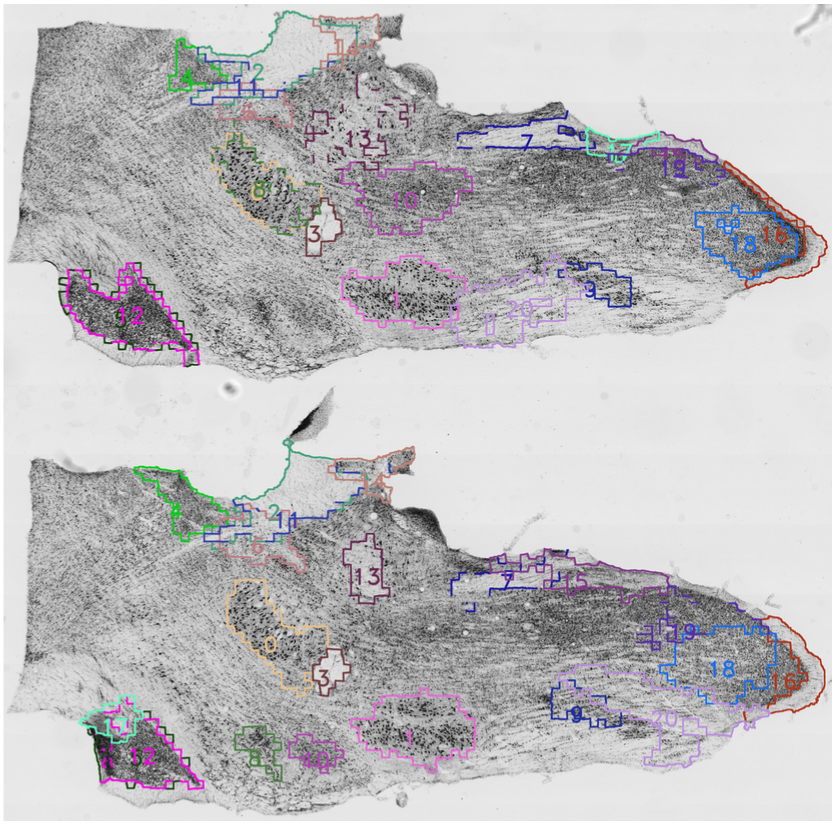
\includegraphics[width=\textwidth]{../figures/MatchedLMs_0006_0007.png}
	\caption{Landmark matching example. Matched landmarks are marked with the same color and number. No position information is used. Notice how matching 13 is made possible by modelling both open boundaries and close boundaries. Many landmarks, for example, 1 and 9, shows considerable shape change, but are still matched.}
	\label{fig:LandmarkMatch}
\end{figure}

%\section{Related Work}
%
%In this section we review relevant work on texture representation and saliency detection.
%
%%\subsection*{Texture Representation}
%%
%%Gabor filters are widely used to model textures. \cite{jain1990unsupervised} used it in texture segmentation. \cite{clausi2000designing} describes the optimal strategy for choosing the frequency spacing to minimize redundancy.
%%
%%Local Spectral histograms
%%
%%Other descriptors that have been applied to histology images include local binary patterns, grey-level co-occurrence matrix, intensity histogram and SIFT. [Tu]
%%
%%Textons are proposed in \cite{leung2001representing}
%
%
%
%\subsection*{Saliency and Objectness Detection}
%
%Our idea of formulating significance as a statistical test 
%
%discriminative saliency \cite{gao2009decision} where hypothesis testing is used with the surround modeled as null.
%
%Other bottom-up approaches for saliency detection based on contrast of histograms \cite{cheng2011global} (Region based contrast)
%
%
%%Detecting significant regions is similar in spirit with a large body of work on saliency detection. These work aim to detect most attract attention
%
%Our use of , especially similar to the bottom-up approaches
%
%top-down approaches rely on detecting high-level objects 
%
%bottom-up approaches directly capture saliency using low-level features.
%
%These include 
%global rarity scheme include
%
%center-surround scheme \cite{perazzi2012saliency}
%\cite{cheng2011global}



%\subsection*{Landmark Detection on Histology Images}
%
%Point landmarks are used 



\section{Conclusion and Future Work}

In this paper we described algorithms for detecting region and boundary landmarks from histology images of mouse brainstem. Region proposals are grown from superpixels, based on which significant regions such as nuclei and fiber tracts are identified using clustering. These regions are shown to correspond well with real anatomical structures. To complement region landmarks, robust boundary segments are also found by consensus voting. Landmarks from different sections can be matched using a distance function that is robust under distortion.

The next step of this project is to use the matched landmarks for intra-specimen registration, and further co-register multiple specimens to generate the atlas.

We plan to explore how to most efficiently use human supervision

We will explore new representations of texture. A promising direction is to learn visual dictionary directly from the images using independent component analysis or deep neural networks.





%
% ---- Bibliography ----
%

\bibliography{bibfile}
\bibliographystyle{splncs03}

%\begin{thebibliography}{5}
%%
%\bibitem {clar:eke}
%Clarke, F., Ekeland, I.:
%Nonlinear oscillations and
%boundary-value problems for Hamiltonian systems.
%Arch. Rat. Mech. Anal. 78, 315--333 (1982)
%
%\bibitem {slic}
%Radhakrishna Achanta, Appu Shaji, Kevin Smith, Aurelien Lucchi, Pascal Fua, and Sabine Süsstrunk, SLIC Superpixels, EPFL Technical Report no. 149300, June 2010.
%
%\end{thebibliography}


\end{document}
